% Chapter Template

\chapter{FDTD - Three-Dimensional Scenario} % Main chapter title

\label{Chapter4} % Change X to a consecutive number; for referencing this chapter elsewhere, use \ref{ChapterX}

%----------------------------------------------------------------------------------------
%	SECTION 1
%----------------------------------------------------------------------------------------

\section{3D Discretization}

\begin{figure}[h!]
	\centering
	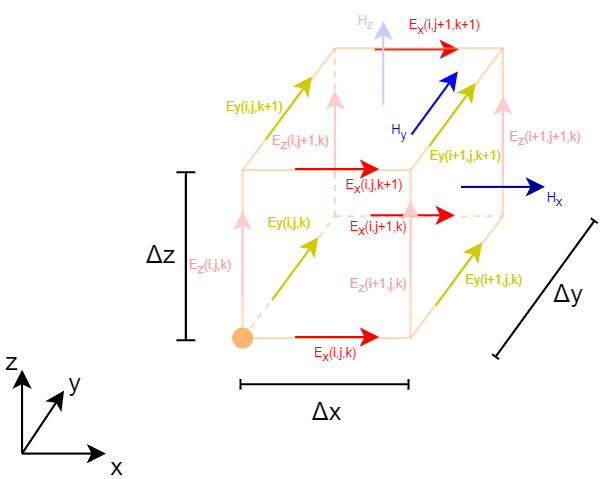
\includegraphics[scale=0.6]{Figures/fdtd3dFull}
	\decoRule
	\caption[3D Electric Discretization]{The figure shows the vectors for the electric field, with the respective magnetic vectors.}
	\label{fig:fdtd3dFull}
\end{figure}

%-----------------------------------
%	SUBSECTION 1
%-----------------------------------
\subsection{3D Electromagnetic Curls}

\begin{figure}[h!]
	\centering
	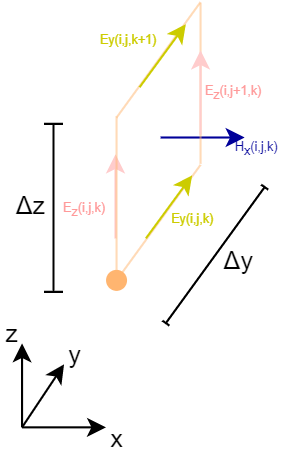
\includegraphics[scale=0.6]{Figures/fdtd3dHxCurl}
	\decoRule
	\caption[3D $H_x$ vector curl]{The curl around the magnetic field vector $H_x$.}
	\label{fig:fdtd3dHxCurl}
\end{figure}


\begin{figure}[h!]
	\centering
	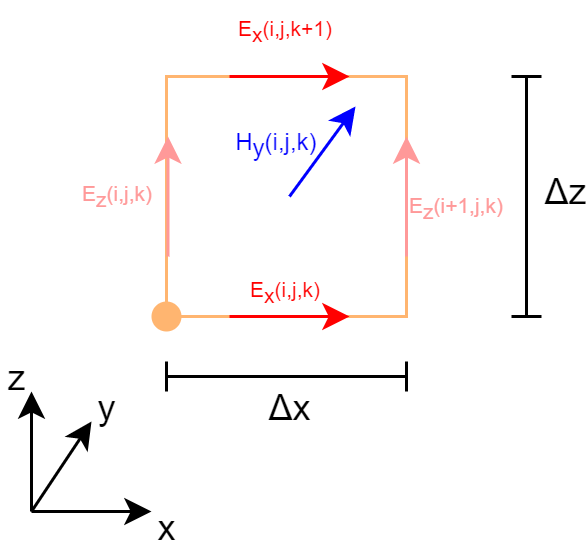
\includegraphics[scale=0.5]{Figures/fdtd3dHyCurl}
	\decoRule
	\caption[3D $H_y$ vector curl]{The curl around the magnetic field vector $H_y$.}
	\label{fig:fdtd3dHyCurl}
\end{figure}

\begin{figure}[h!]
	\centering
	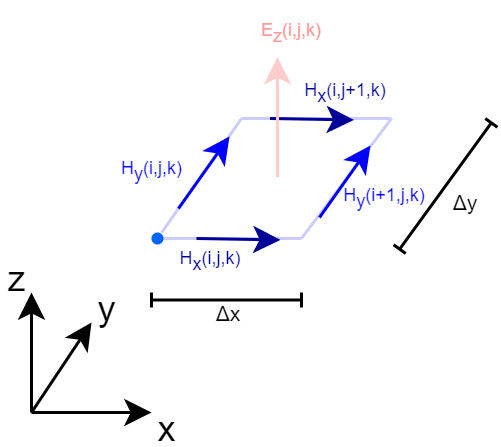
\includegraphics[scale=0.5]{Figures/fdtd3dEzCurl}
	\decoRule
	\caption[3D $E_z$ vector curl]{The curl around the electric field vector $E_z$.}
	\label{fig:fdtd3dEzCurl}
\end{figure}




%----------------------------------------------------------------------------------------
%	SECTION 2
%----------------------------------------------------------------------------------------

\section{C++ Implementation}

\section{Data Visualization}

\begin{figure}[h!]
	\centering
	\begin{subfigure}{.49\textwidth}
		\centering
		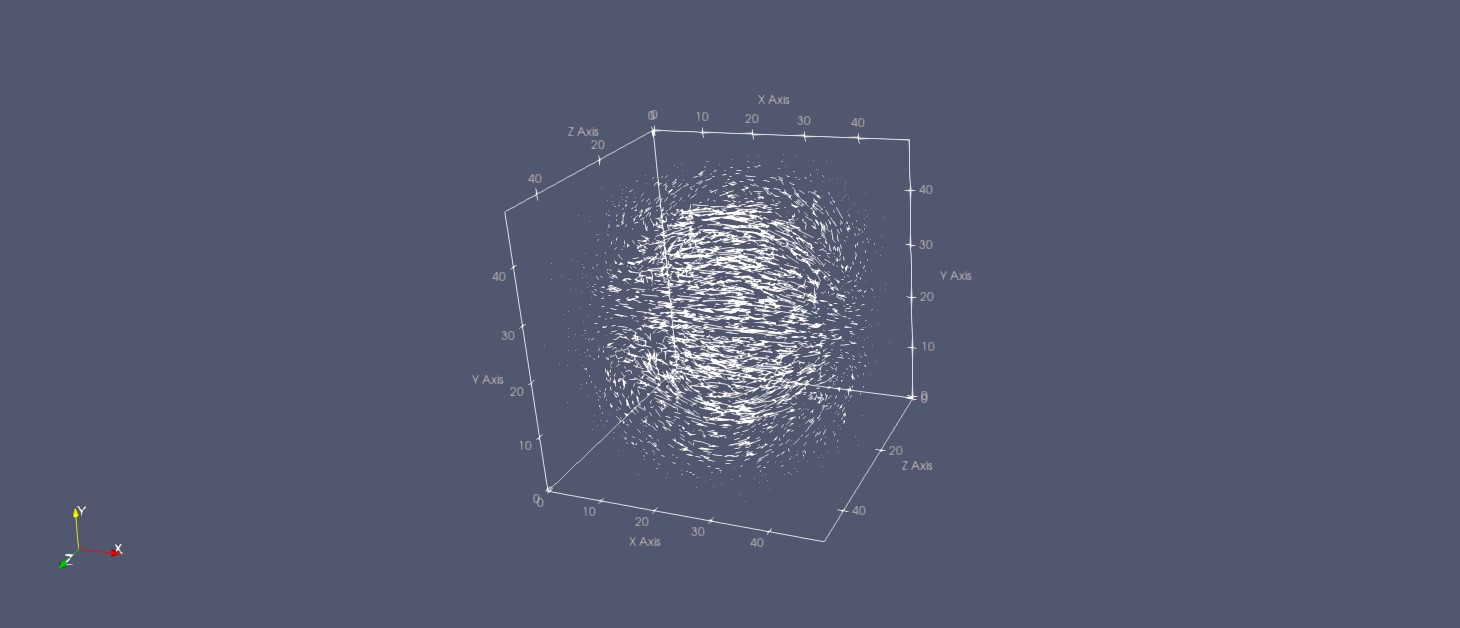
\includegraphics[width=.95\linewidth]{Figures/FDTD3DE1}
		\caption{t = 50}
	\end{subfigure}
	\begin{subfigure}{.49\textwidth}
		\centering
		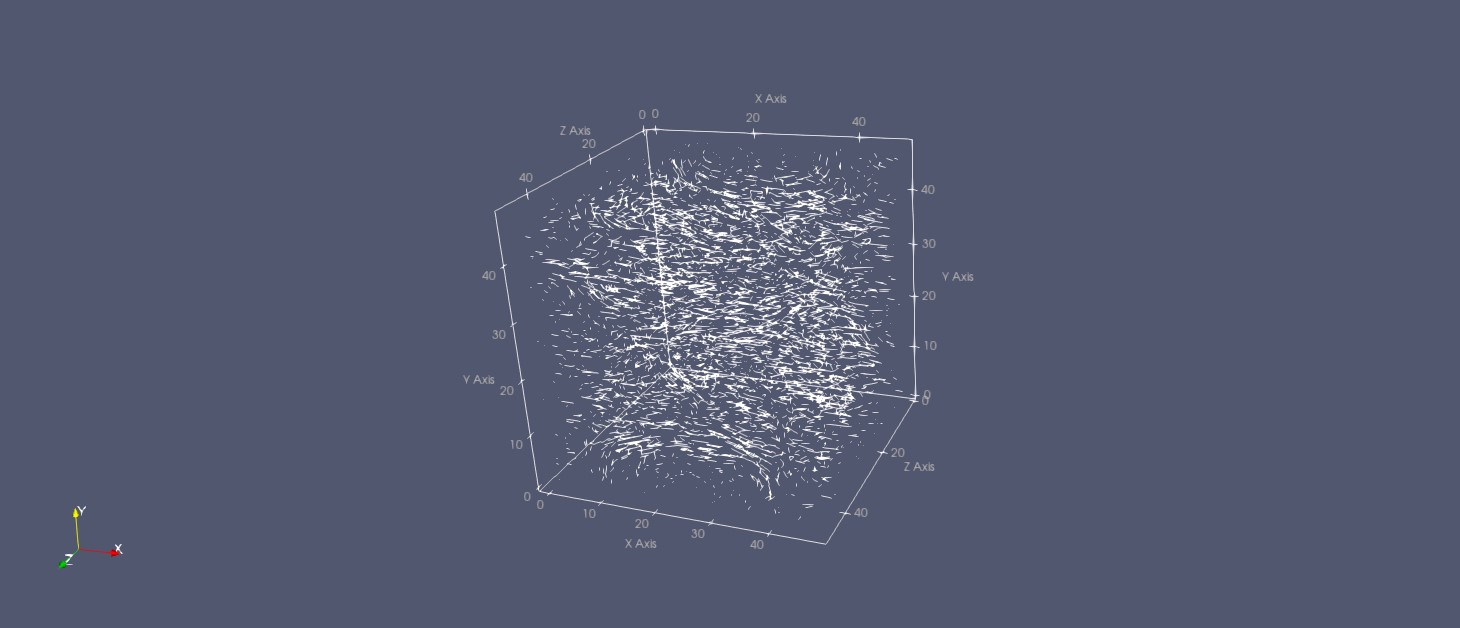
\includegraphics[width=.95\linewidth]{Figures/FDTD3DE2}
		\caption{t = 100}
	\end{subfigure}
	\begin{subfigure}{.49\textwidth}
		\centering
		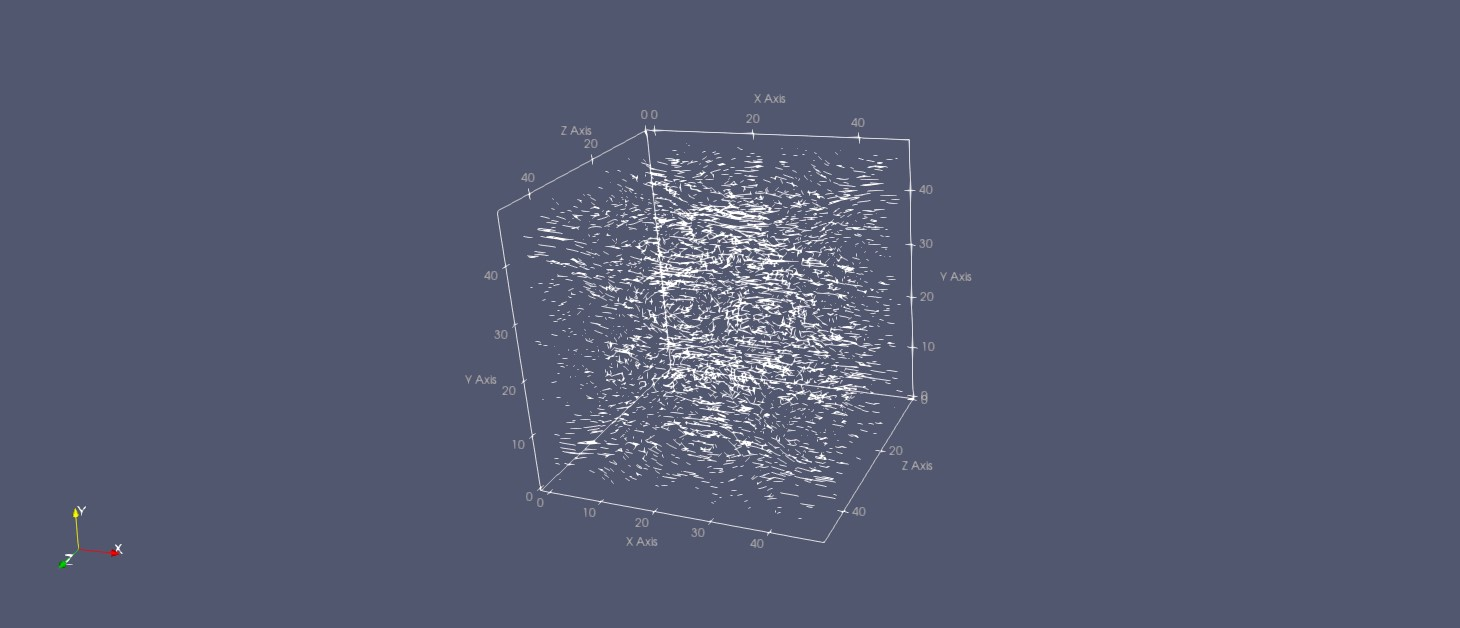
\includegraphics[width=.95\linewidth]{Figures/FDTD3DE3}
		\caption{t = 150}
	\end{subfigure}
	\begin{subfigure}{.49\textwidth}
		\centering
		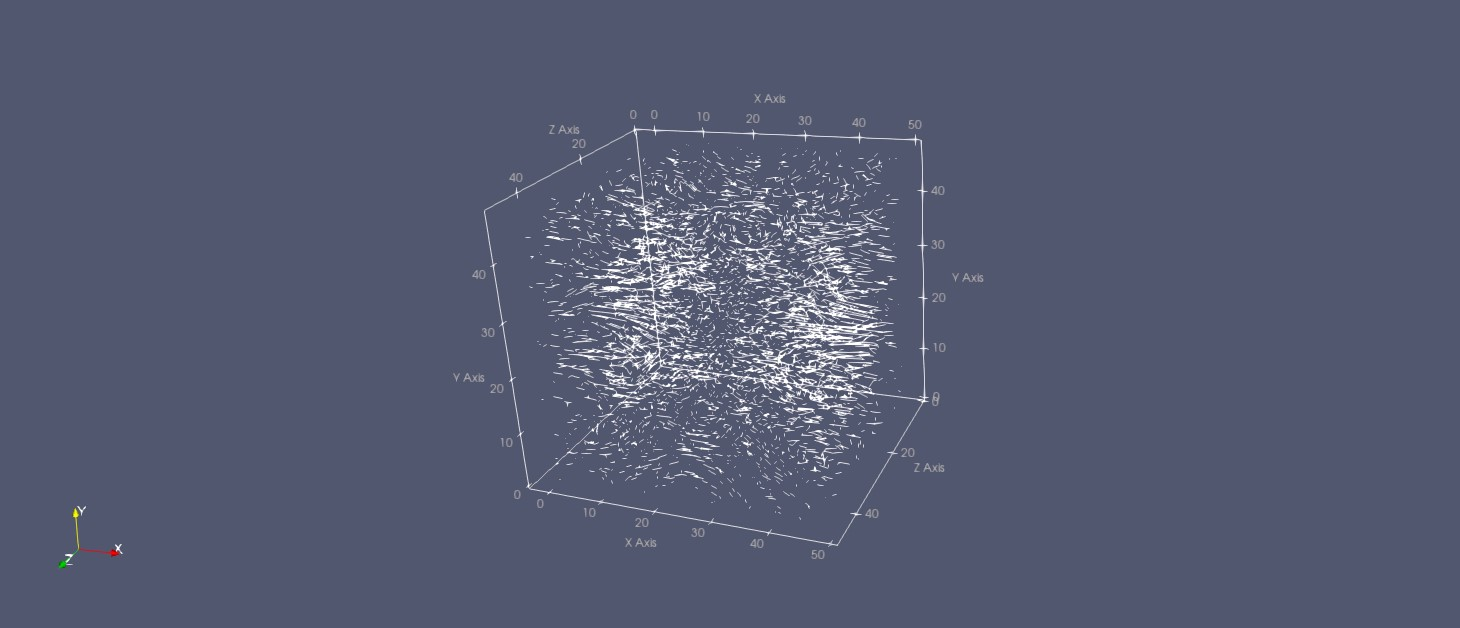
\includegraphics[width=.95\linewidth]{Figures/FDTD3DE4}
		\caption{t = 200}
	\end{subfigure}
	\decoRule
	\caption[3D Electric Field Simulation]{A simulation of the 3D electric field.}
	\label{fig:FDTD3DE}
\end{figure}

\begin{figure}[h!]
	\centering
	\begin{subfigure}{.49\textwidth}
		\centering
		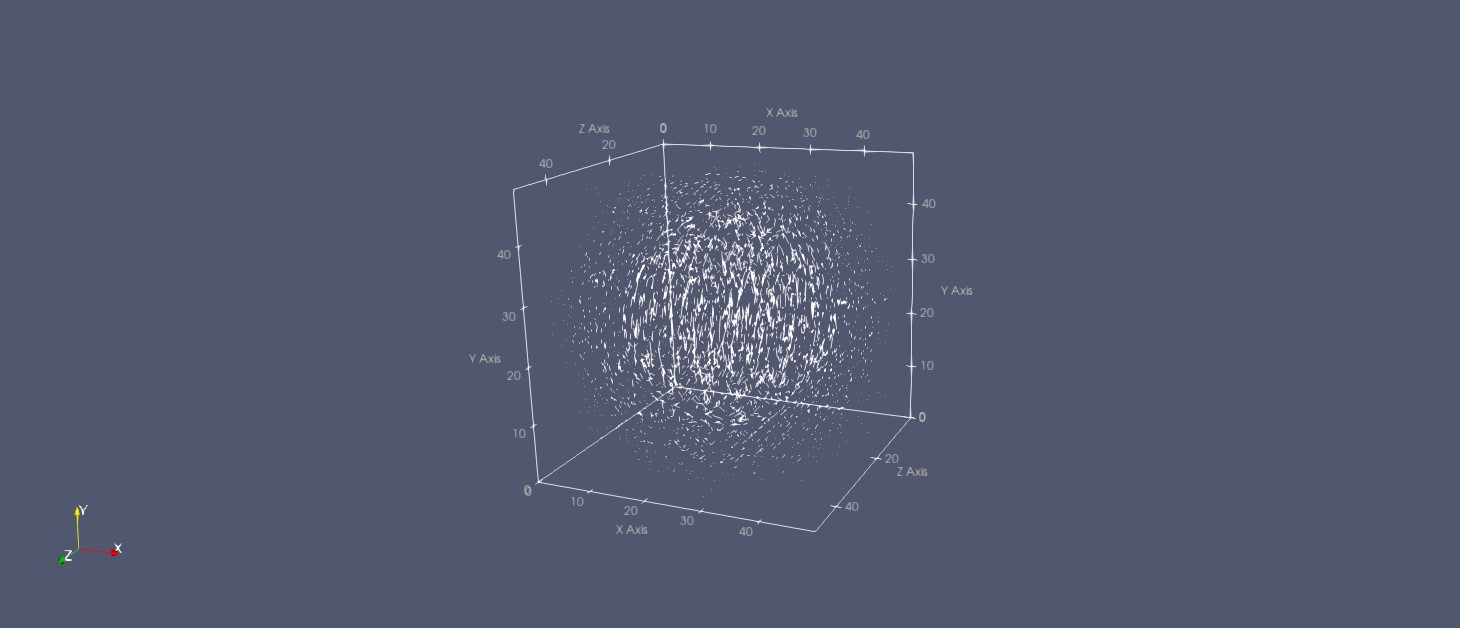
\includegraphics[width=.95\linewidth]{Figures/FDTD3DH1}
		\caption{t = 200}
	\end{subfigure}
	\begin{subfigure}{.49\textwidth}
		\centering
		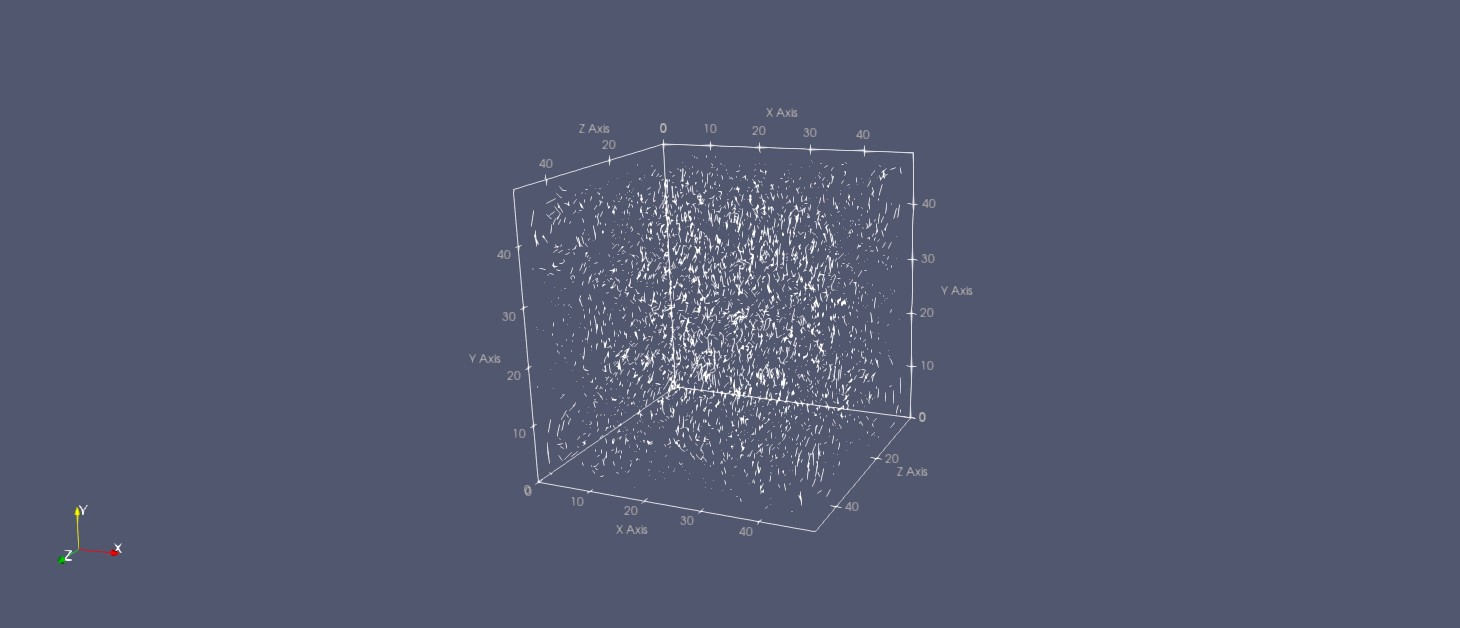
\includegraphics[width=.95\linewidth]{Figures/FDTD3DH2}
		\caption{t = 400}
	\end{subfigure}
	\begin{subfigure}{.49\textwidth}
		\centering
		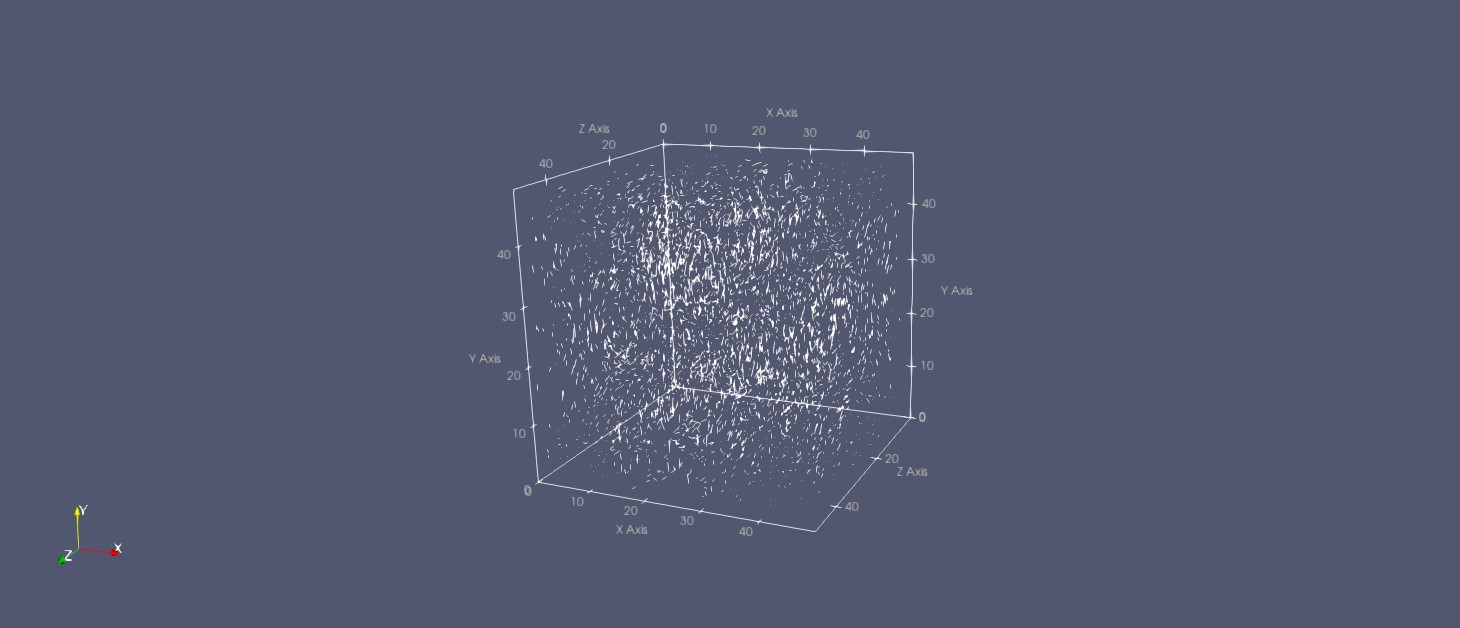
\includegraphics[width=.95\linewidth]{Figures/FDTD3DH3}
		\caption{t = 600}
	\end{subfigure}
	\begin{subfigure}{.49\textwidth}
		\centering
		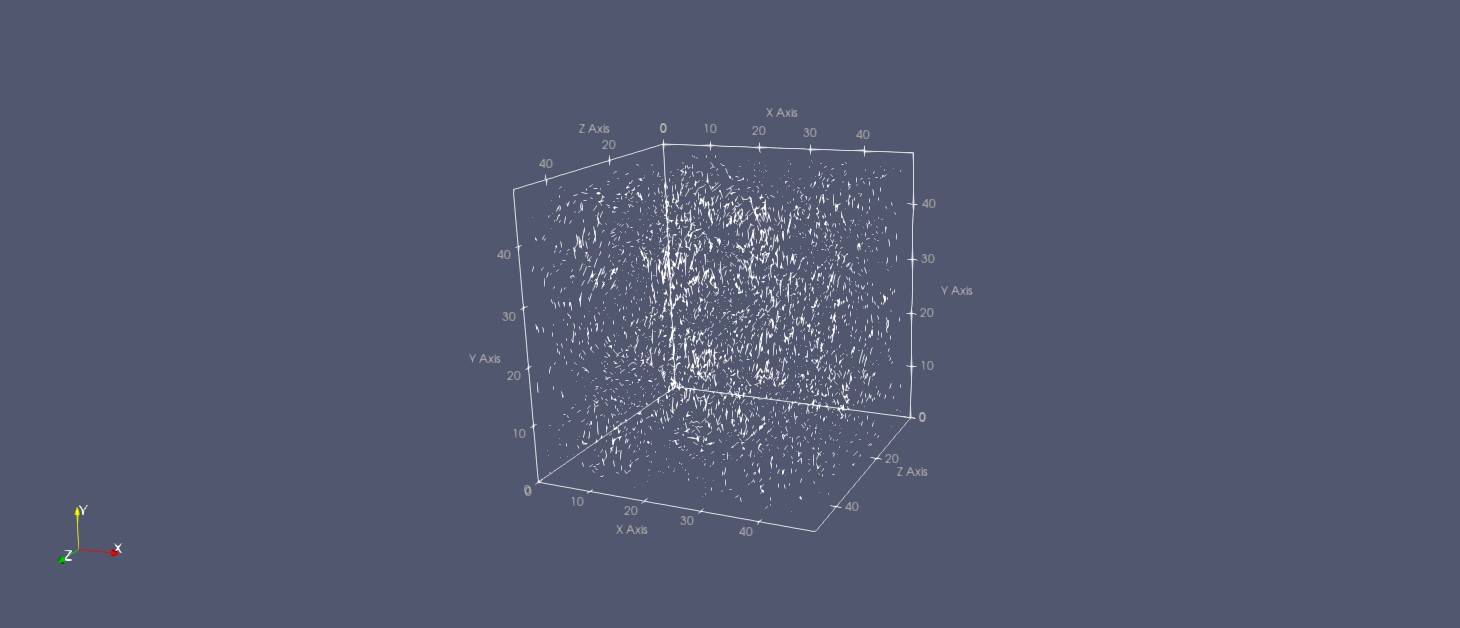
\includegraphics[width=.95\linewidth]{Figures/FDTD3DH4}
		\caption{t = 800}
	\end{subfigure}
	\decoRule
	\caption[3D Magnetic Field Simulation]{A simulation of the 3D magnetic field.}
	\label{fig:FDTD3DH}
\end{figure}